\documentclass[hyperref=unicode]{beamer}

\usepackage[absolute,overlay]{textpos}
\usepackage{graphicx}
\usepackage{adjustbox}
\usepackage{chemfig}
\usepackage[version=4]{mhchem}
\usepackage{wrapfig}
\usepackage{multirow}
\adjustboxset*{center}
\usepackage{caption}
\usepackage{chemformula}
\usepackage{elements}

%dělení slov
\usepackage{ragged2e}
\let\raggedright=\RaggedRight
%konec dělení slov

\usepackage{fontspec}
\usepackage{unicode-math}

\usepackage{polyglossia}
\setdefaultlanguage{czech}

\def\uv#1{„#1“}

\mode<presentation>{\usetheme{Madrid}}
\DefineNamedColor{named}{pozadi}{RGB}{200,200,200}
\usecolortheme{crane}

\setbeamertemplate{footline}[frame number]

\addtobeamertemplate{frametitle}{
	\let\insertframetitle\insertsectionhead}{}
\addtobeamertemplate{frametitle}{
	\let\insertframesubtitle\insertsubsectionhead}{}

\makeatletter
\CheckCommand*\beamer@checkframetitle{\@ifnextchar\bgroup\beamer@inlineframetitle{}}
\renewcommand*\beamer@checkframetitle{\global\let\beamer@frametitle\relax\@ifnextchar\bgroup\beamer@inlineframetitle{}}
\makeatother
\setbeamercolor{section in toc}{fg=blue}
\setbeamertemplate{section in toc shaded}[default][100]

\usepackage{tikz}
\usetikzlibrary{positioning}
\usetikzlibrary{arrows}
\usetikzlibrary{shapes.multipart}

\usepackage{tikz-3dplot}
\usetikzlibrary{decorations}
\usepackage{multirow}
\usepackage{gensymb}
\usepackage{textcomp}
\pgfdeclarelayer{background}
\pgfdeclarelayer{foreground}

\title[Crisis]
{Orbitaly, VSEPR}

\subtitle{Rezonanční struktury, atomové a molekulové orbitaly, hybridizace, určování tvaru molekuly pomocí teorie VSEPR, úvod do symetrie molekul, dipólový moment}

%\author{Zdeněk Moravec, \href{http://z-moravec.net/chemie/zaklady-chemie/}{http://z-moravec.net}}
\author{Zdeněk Moravec, hugo@chemi.muni.cz}

\date{}
\begin{document}

\frame{\titlepage}

\section{Formální náboj}
\frame{
	\frametitle{}
	\begin{itemize}
	\item Rozdíl mezi počtem valenčních elektronů ve volném atomu a valenčních elektronů ve vázaném atomu.
	\item Záporný náboj je umístěn na nejelektronegativnějším atomu.
	\item Součet formálních nábojů všech atomů v molekule je roven jejímu náboji.
	\item \ce{H3O^+}: H: 0; O: 6-5=+1
	\item \ce{CH3^+}: H: 0; C: 4-3=+1
	\end{itemize}
	\begin{center}
	\adjincludegraphics[width=80mm]{formalni_naboj.png}
	\end{center}
}

\section{Rezonanční struktury}
\frame{
	\frametitle{}
	\begin{itemize}
	\item Popisují polohu elektronů v molekulách.
	\item Vyjadřují jednotlivé limitní stavy.
	\end{itemize}
	\begin{center}
	\schemestart
	\rotatebox{30}{\chemfig{*6(=-=-=-)}}\arrow{<=>}\rotatebox{30}{\chemfig{*6(=-=-=-)}}
	\schemestop
	\end{center}
	\scalebox{0.7}{
	\schemestart
	\chemfig{S(-[:0]O^{\scriptstyle -})(=[:90]O)(-[:180]^{\scriptstyle -}O)(=[:270]O)}\arrow{<=>}
	\chemfig{S(-[:0]O^{\scriptstyle -})(=[:90]O)(=[:180]O)(-[:270]\chembelow{O}{\scriptstyle -})}\arrow{<=>}
	\chemfig{S(=[:0]O)(-[:90]\chemabove{O}{\scriptstyle -})(=[:180]O)(-[:270]\chembelow{O}{\scriptstyle -})}\arrow{<=>}
	\chemfig{S(=[:0]O)(=[:90]O)(-[:180]^{\scriptstyle -}O)(-[:270]\chembelow{O}{\scriptstyle -})}
	\schemestop
	}
}

\section{Atomové orbitaly}
\frame{
	\frametitle{}
	\begin{itemize}
	\item Funkce popisující prostorové rozložení pravděpodobnosti výskytu elektronu.
	\item Orbitaly jsou popsány třemi kvantovými čísly.
	\begin{itemize}
	\item Hlavní kvantové číslo (n) - popisuje příslušnost orbitalu do elektronové slupky -- velikost orbitalu. Nabývá hodnot větších než 0.
	\item Vedlejší kvantové číslo (l) - popisuje tvar orbitalu. Často se používá označení pomocí písmen: s, p, d, f, g, h, ... Nabývá hodnot v intervalu $<0, n-1>$.
	\item Magnetické kvantové číslo (m) - popisuje prostorovou orientaci orbitalu. Nabývá hodnot v intervalu $<-l; l>$.
	\item {\color{gray}Spinové kvantové číslo (s) - nepopisuje orbital, ale spin elektronu v orbitalu. Nabývá hodnot $\pm$\textonehalf.}
	\end{itemize}
	\item \textbf{Nodální rovina} - rovina, kde je pravděpodobnost výskytu elektronu nulová, vlnová funkce orbitalu mění při průchodu touto rovinou znaménko.
	\end{itemize}
	\footnotetext[1]{\href{http://www.chemguide.co.uk/atoms/properties/atomorbs.html}{www.chemguide.co.uk/atoms/properties/atomorbs.html}}
}

\frame{
	\frametitle{}
	\begin{itemize}
	\item Orbital s - kulově symetrický, magnetické číslo je vždy rovno 0. Tyto orbitaly mají $n-1$ kulových nodálních ploch.
	\item Orbital p - středově symetrický tvar, skládající se ze dvou laloků. V místě spojení laloků je nodální plocha, kde vlnová funkce popisující orbital mění znaménko. Magnetické kvantové číslo pro orbital p nabývá hodnot: -1, 0, 1.
	\item Orbital d - existuje pět typů orbitalů d, tři meziosé, jejichž laloky leží mezi osami souřadného systému - $d_{xy}$, $d_{xz}$ a $d_{zy}$. Orbital $d_{x^2-y^2}$ má čtyři laloky umístěné v osách x a y. Poslední orbital, $d_{z^2}$ má dva laloky umístěné v ose z a prstenec, ležící v rovině xy.
	\end{itemize}
	\adjincludegraphics[width=105mm]{orbitals-new.pdf}
}

\frame{
	\frametitle{}
	\begin{itemize}
	\item Orbital f - existuje sedm degenerovaných orbitalů typu f. Tyto orbitaly jsou obsazovány elektrony až u vnitřně přechodných prvků.
	\end{itemize}

	\begin{center}
	\adjincludegraphics[width=85mm]{forbitals.png}
	\url{https://commons.wikimedia.org/wiki/File:F\_orbital.png}
	Autor: \href{https://commons.wikimedia.org/wiki/User:A2569875}{A2569875}
	\end{center}
}

\section{Molekulové orbitaly}
\frame{
	\frametitle{}
	\begin{itemize}
	\item Teorie LCAO-MO - Linear Combination of Atomic Orbitals - Molecular Orbital.
	\item Molekulové orbitaly vznikají lineární kombinací atomových orbitalů.
	\item Kombinací dvou AO vznikají dva MO - vazebný a protivazebný. Protivazebné orbitaly se označují hvězdičkou, např. $\sigma^*$.
	\item Aby byl překryv úspěšný musí mít vlnové funkce orbitalů v místě překryvu stejná znaménka.
	\item Protivazebný orbital má o jednu nodální plochu více než vazebný a pokud je obsazen elektronovým párem, snižuje řád vazby o jedna. Obsazený vazebný orbital naopak řád vazby zvyšuje.
	\item Vazba $\sigma$ - vzniká osovým překryvem orbitalů.
	\item Vazba $\pi$ - vzniká bočným překryvem orbitalů, je přítomna v násobných vazbách.
	\item Vazba $\delta$ - vzniká překryvem všech čtyř laloků d-orbitalu, je přítomna ve čtverné vazbě např. v \href{http://pubs.acs.org/doi/abs/10.1021/ic50025a015}{\ce{[Re2Cl8]^{2-}}}.
	\end{itemize}
	\footnotetext[1]{\href{http://chemed.chem.purdue.edu/genchem/topicreview/bp/ch8/mo.html}{Molecular Orbital Theory}}
}

\frame{
	\frametitle{}
	\begin{columns}
	\begin{column}{0.4\textwidth}
	\adjincludegraphics[width=28mm]{2nd_row_diatomic_MOs.jpg}
	\end{column}
	\begin{column}{0.6\textwidth}
	\begin{flushleft}
	Molekulové orbitaly v \ce{O2}
	\newline
	Zdroj: \href{https://commons.wikimedia.org/wiki/File:2nd\_row\_diatomic\_MOs.jpg}{https://commons.wikimedia.org/}
	\newline
	Autor: \href{https://commons.wikimedia.org/wiki/User:Tem5psu}{Tem5psu}
	\end{flushleft}
	\end{column}
	\end{columns}
}


\section{Řád vazby}
\frame{
	\frametitle{Řád vazby}
	\begin{itemize}
	\item Řád vazby popisuje počet elektronových párů, které tvoří vazbu mezi atomy.
	\item Lze jej odvodit z Lewisovského vzorce molekuly nebo z diagramu MO.
	\end{itemize}

	\begin{center}
	\chemfig{H-[:52.24]\charge{45=\:,135=\:}{O}-[::-104.48]H}
	\raisebox{3.5ex}{\chemfig{\charge{90=\:,270=\:}{O}=C=\charge{90=\:,270=\:}{O}}}
	\end{center}

	\begin{itemize}
	\item Řád vazby lze spočítat z počtu elektronů ve vazebných a protivazebných orbitalech.
	\item $RV = \frac{vazebne\ elektrony - protivazebne\ elektrony}{2}$

	\item Neobsazené molekulové orbitaly neovlivňují ani řád vazby, ani energii systému.
	\end{itemize}

}

\section{Oktetové pravidlo}
\frame{
	\frametitle{}
	\begin{itemize}
		\item Nepřechodné prvky se snaží vytvářet chemické vazby tak, aby měly ve valenční slupce osm elektronů, čímž dosáhnou na elektronovou konfiguraci vzácného plynu.
		\item Elektrony, které atomy sdílí v kovalentních vazbách se započítávají pro každý atom zvlášť. Např. v molekule \ce{CO2} jsou kyslíky obklopeny čtyřmi nevazebnými elektrony a~čtyři vazebnými, centrální uhlík je pak obklopen celkem osmi elektrony ze čtyř kovalentních vazeb.
	\end{itemize}

	\begin{center}
		\chemfig{{\charge{90=\:,270=\:}{O}=C=\charge{90=\:,270=\:}{O}}}
	\end{center}

	\begin{itemize}
		\item Existuje několik výjimek z oktetového pravidla, u nekovů z třetí a~vyšší periody se setkáváme s tzv. \textit{elektronovým dodecetem}, kdy má atom ve valenční slupce 12 elektronů. Toho může dosáhnout díky nezaplněným d-orbitalům.
		\begin{itemize}
			\item Příkladem je molekula \ce{ICl5}, kde má jód dva nevazebné elektrony a~celkem 10 elektronů z pěti kovalentních vazeb.
			\item Podobně síra v molekule \ce{SF6} má ve valenční slupce celkem 12~elektronů ze šesti kovalentních vazeb \ce{S-F}.
		\end{itemize}
	\end{itemize}
}

\section{Hybridizace}
\frame{
	\frametitle{}
\begin{itemize}
	\item Hybridizace atomových orbitalů --- proces energetického mísení a směrového vyrovnání atomových orbitalů daného atomu
	\item Počet hybridních orbitalů odpovídá počtu mísených atomových orbitalů
\end{itemize}
\begin{tabular}{|l|l|}
\hline
\textbf{Hybridizace} & \textbf{Geometrie molekuly} \\
\hline
sp & lineární \\
\hline
sp$^2$ & rovnostranný trojúhelník \\
\hline
sp$^3$ & tetraedr \\
\hline
d$^2$sp$^3$ & oktaedr \\
\hline
dsp$^2$ & čtverec \\
\hline
\multirow{2}{*}{dsp$^3$} & trigonální bipyramida \\
& čtvercová pyramida \\
\hline
\end{tabular}
\footnotetext[1]{\href{http://www.science.uwaterloo.ca/~cchieh/cact/c120/hybrid.html}{Valence Bond Theory and Hybrid Atomic Orbitals}}
}

\section{VSEPR}
\frame{
	\frametitle{}
	\begin{itemize}
	\item \textbf{V}alence \textbf{S}hell \textbf{E}lectron \textbf{P}air \textbf{R}epulsion
	\item Tvar molekuly určíme na základě rozmístění elektronových párů v okolí centrálního atomu tak, aby jejich vzájemné odpuzování bylo co nejmenší.
	\item Tento model je vhodný převážně pro sloučeniny nepřechodných prvků.
	\item Uvažujeme pouze nevazebné elektronové páry - $n$ a vazebné elektronové páry $\sigma$.
	\item \textbf{Základní pravidla VSEPRu}
	\begin{enumerate}
		\item Elektronové páry centrálního atomu se v prostoru rozmístí tak, aby byly co nejdále od sebe a měly minimální energii.
		\item Nevazebný elektronový pár odpuzuje ostatní elektronové páry nejvíce, odpuzování  vazebných elektronových párů je slabší a klesá v pořadí trojná vazba $>$ dvojná vazba $>$ jednoduchá vazba.
		\item Tvar molekuly je dán pouze polohou vazebných elektronových párů.
	\end{enumerate}
	\end{itemize}
	\footnotetext[1]{ \href{http://www.chemvazba.moxo.cz/Lekce/lekce5.html}{Teorie VSEPR}}
}

\subsection{Výchozí tvary}
\frame{
	\frametitle{}
	\begin{tabular}{|c|c|c|}
	\hline
	Počet elektronových párů & \multicolumn{2}{|c|}{Tvar} \\\hline
	2 & lineární &\color{red} X---A---X \\\hline
	3 & trojúhelník &  \raisebox{-.9\height}{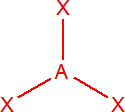
\includegraphics[width=20mm]{AX3.png}} \\[40pt]
	\hline
	4 & tetraedr & \raisebox{-.9\height}{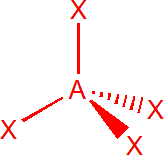
\includegraphics[width=20mm]{AX4.png}} \\[40pt]
	\hline
	\end{tabular}
}

\frame{
	\frametitle{}
	\begin{tabular}{|c|c|c|}
	\hline
	Počet elektronových párů & \multicolumn{2}{|c|}{Tvar} \\\hline
	5 & trigonální bipyramida & \raisebox{-.9\height}{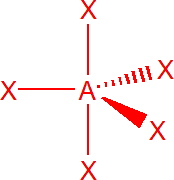
\includegraphics[width=20mm]{AX5.png}} \\[65pt]
	\hline
	6 & oktaedr & \raisebox{-.9\height}{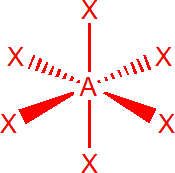
\includegraphics[width=20mm]{AX6.png}} \\[65pt]
	\hline
	\end{tabular}
}

\subsection{Dva elektronové páry na centrálním atomu}
\frame{
	\frametitle{}
Pokud centrální atom (A) nese dva elektronové páry, je tvar molekuly vždy lineární. Pokud jsou oba vazebné (X), označujeme molekulu jako \ce{AX2}, pokud je jeden nevazebný (E), označení je \ce{AXE}.
\\
\hrule
\vspace{5mm}
\ce{AX2}
\\
\vspace{5mm}
{\LARGE\color{red} X---A---X}
\vspace{5mm}

Tvar: lineární; $\angle XAX = 180\degree$; Příklad: \ce{CO2}, \ce{BeF2}
\vspace{5mm}
\hrule
\vspace{5mm}
\ce{AXE}

\vspace{5mm}
{\LARGE E---\color{red} A---X}
\vspace{5mm}


Tvar: lineární; $\angle EAX = 180\degree$;  Příklad: CO
}

\subsection{Tři elektronové páry na centrálním atomu}
\frame{
	\frametitle{}

\ce{AX3}

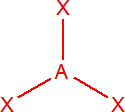
\includegraphics[width=30mm]{AX3.png}

Tvar:  rovnostranný trojúhelník; $\angle XAX = 120\degree$
Příklad: \ce{BCl3}
}

\frame{
	\frametitle{}

\ce{AX2E}
\begin{columns}
\column{.35\textwidth}
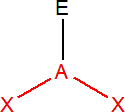
\includegraphics[width=30mm]{AX2E.png}
\column{.65\textwidth}
Tvar: lomený; $\angle XAX < 120\degree$
Příklad: \ce{SO2}
\end{columns}
\vspace{5mm}
\hrule
\vspace{2mm}
\ce{AXE2}
\begin{columns}
\column{.35\textwidth}
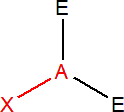
\includegraphics[width=30mm]{AXE2.png}
\column{.65\textwidth}
Tvar: lineární; Příklad: \ce{O2}
\end{columns}
}

\subsection{Čtyři elektronové páry na centrálním atomu}
\frame{
	\frametitle{}
\begin{tabular}{|c|c|c|}
\ce{AX4} & \ce{AX3E} & \ce{AX2E2} \\
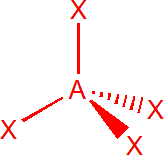
\includegraphics[width=25mm]{AX4.png} &
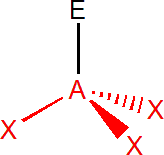
\includegraphics[width=25mm]{AX3E.png} &
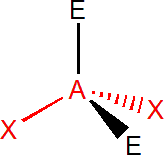
\includegraphics[width=25mm]{AX2E2.png} \\
Tvar: tetraedr & trigonální pyramida & lomený \\
$\angle XAX = 109.5\degree$ & $\angle XAX < 109.5\degree$ & $\angle XAX << 109.5\degree$ \\
Příklad: \ce{SO^{2-}_4} & \ce{PH3} &  \ce{SeBr2} \\
\end{tabular}
}

\subsection{Pět elektronových párů na centrálním atomu}
\frame{
	\frametitle{}
\scalebox{0.93}{
\begin{tabular}{|c|c|c|c|}
\ce{AX5} & \ce{AX4E} & \ce{AX3E2} & \ce{AX2E3} \\
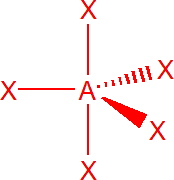
\includegraphics[width=20mm]{AX5.png} &
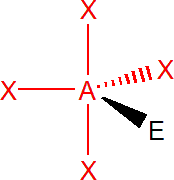
\includegraphics[width=20mm]{AX4E.png} &
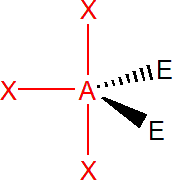
\includegraphics[width=20mm]{AX3E2.png} &
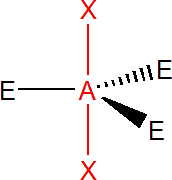
\includegraphics[width=20mm]{AX2E3.png} \\

Tvar: trigonální  & houpačka & tvar T & lineární \\
bipyramida &&&\\
$ 90\degree\ a\ 120\degree$ & $ < 90\degree$ a $< 120\degree$ & $90\degree$
& $180\degree$ \\
Příklad: \ce{AsF5} & \ce{SeH4} &  \ce{ICl3} &  \ce{BrF2^-} \\
\end{tabular}
}%end scalebox
}

\subsection{Šest elektronových párů na centrálním atomu}
\frame{
	\frametitle{}
\begin{tabular}{|c|c|c|}
\ce{AX6} & \ce{AX5E} & \ce{AX4E2} \\
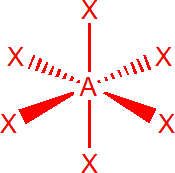
\includegraphics[width=25mm]{AX6.png} &
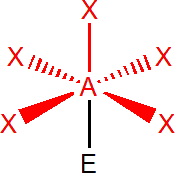
\includegraphics[width=25mm]{AX5E.png} &
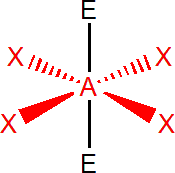
\includegraphics[width=25mm]{AX4E2.png} \\
Tvar: oktaedr & čtvercová pyramida & čtverec \\
$\angle XAX = 90\degree$ & $\angle XAX < 90\degree$ & $\angle XAX = 90\degree$ \\
Příklad: \ce{SF6} & \ce{IF5} &  \ce{XeF4} \\
\end{tabular}
}

\section{Symetrie molekul}
\frame{
	\frametitle{}
	\vfill
	\begin{itemize}
	\item \textbf{Operace symetrie} - geometrická operace, jejímž provedením dostaneme objekt do polohy nerozlišitelné od výchozí.
	\item \textbf{Prvek symetrie} - body, jejichž poloha se v průběhu provádění operace symetrie nemění.
	\item U molekul existuje pět prvků symetrie.
	\end{itemize}

	\begin{tabular}{|l|l|l|}
	\hline
	\textbf{Operace symetrie} & \textbf{Symbol} & \textbf{Prvek symetrie} \\
	\hline
	Identita & E & Celý objekt \\
	\hline
	Rotace & $C_n$ & Rotační osa \\
	\hline
	Zrcadlení & $\sigma$ & Rovina symetrie \\
	\hline
	Inverze & i & Střed symetrie \\
	\hline
	Nevlastní osa & $S_n$ & Rotačně-reflexní osa \\
	\hline
	\end{tabular}
	\vfill
}

\section{Dipólový moment}
\frame{
	\frametitle{}
	\vfill
	\begin{itemize}
	\item Vektor popisující rozložení elektrického náboje v molekule.
	\item Výsledný dipólmoment získáme vektorovým součtem dipólmomentů jednotlivých vazeb.
	\end{itemize}
\begin{columns}
\column{0.6\textwidth}
\begin{center}
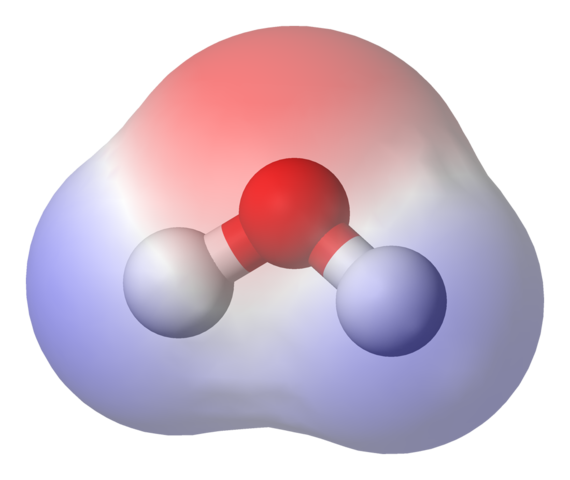
\includegraphics[width=5cm]{water-elpot.png}
\end{center}

\column{0.4\textwidth}
\begin{center}
\begin{picture}(0,0)
\color{red}
\put(0,0){O}
\color{blue}
\put(23,-30){H}
\put(-23,-30){H}
\color{black}
\thicklines
\put(4,-1){\vector(-1,-1){20}}
\put(4,-1){\vector(1,-1){20}}
\put(4,-1){\vector(0,-1){40}}
\thinlines
\put(24,-21){\line(-1,-1){20}}
\put(-16,-21){\line(1,-1){20}}
\end{picture}
\end{center}
\end{columns}
	\vfill
}

\end{document}